\section{Morfometria del bacino}
\subsection{Rapporto di biforcazione e prima legge di Horton}
Secondo la prima legge di Horton, il rapporto tra la numerosità dell'ordine precedente e la numerosità dell'ordine considerato (detto ``rapporto di biforcazione parziale")
\begin{equation}
    R_u = \frac{N_{u-1}}{N_u}
\end{equation}
è statisticamente costante, e regolata dalla funzione:
\begin{equation}
    N_u= \bar{R}_b ^{(k-u)}
\end{equation}
Dove: 
\begin{itemize}
    \item $R_b$ è la media tra i rapporti di biforcazione parziali;
    \item $k$ è l'ordine del bacino, nel caso di quello preso in considerazione il valore è 3;
    \item $u$ è l'ordine del tratto di reticolo considerato.
\end{itemize}
La prima legge di Horton inoltre, evidenzia come all'aumentare dell'ordine dei tratti, la lunghezza dei segmenti e le aree dei sottobacini aumentino, mentre cala la loro numerosità.\\
Nel caso del reticolo idrografico preso da noi in esame, i parametri sono: 

\begin{table}[H] \centering
    \caption{\textcolor{red}{Caratteristiche di biforcazione del reticolo idrografico ed applicazione della prima legge di Horton}}
    \label{tab:rapp_biforcazione_1_horton}
    \begin{tabular}{ cccc }
\toprule
    Ordine u & Segmenti Nu & Rapp. di biforcazione Rb & Nu (prima legge di Horton) \\
\midrule    
    1        & 5           &   /                     & 5.1                        \\
    2        & 2           & 2.5                      & 2.3                        \\
    3        & 1           & 2.0                      & 1.0                       \\
\bottomrule    
\end{tabular}
\end{table}
Il rapporto di biforcazione medio $\bar{R}_b$ è pari a \num{2.3}.\\
Interpolando i valori degli ordini dei segmenti, con la loro numerosità e con il parametro ricavato dalla prima legge di Horton, si ottiene un grafico caratteristico:
\begin{figure}[H]\centering
    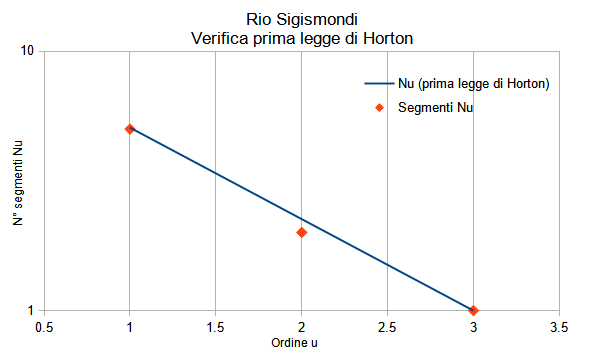
\includegraphics[scale=.75]{immagini/legge_horton.png}
    \caption{Relazione tra l'ordine del tratto, la sua numerosità e la funzione di Horton.}
    \label{legge_horton}
\end{figure}

\subsection{Coefficiente di forma di Gravelius}
Il coefficiente di forma di Gravelius è un parametro che indica quanto la forma di un bacino sia compatta.\\
Questo indicatore confronta le misure di area e perimetro del bacino in analisi, con le misure che avrebbe un cerchio di uguale superficie; quindi, più l'indice tende ad uno e maggiore sarà la compattezza dell'area studiata.\\
Al fine di applicare la relativa formula, è necessario conoscere i valori di perimetro del bacino (lunghezza dello spartiacque), e l'area della superficie dell'intera area di studio.\\
La formula dell'indicatore è:
\begin{equation}
    F = \frac{0.28 \cdot P}{\sqrt{A}}
    \label{gravelius}
\end{equation}

\subsection{Indice di compattezza $F_c$}
Proprio come per l'indice precedente, questa formula permette di comprendere la forma del bacino.\\
Al contrario del coefficiente precedente, che utilizza il valore del perimetro, questa formula necessita di conoscere la lunghezza del reticolo idrografico del bacino, oltre che alla superficie drenante interna allo spartiacque.\\
La formula dell'indicatore è:
\begin{equation}
    F_c = \frac{L}{\sqrt{A}}
    \label{compatezza}
\end{equation}

\subsection{Indice di Melton}
L'indice di Melton quantifica l'energia potenziale (gravitativa) del bacino.\\
La formula è applicabile conoscendo il dislivello di quota tra quella massima del bacino e quella dell'apice del cono di deiezione, oltre che l'area totale del bacino. 
\begin{equation}
    Me = \frac{\Delta H}{\sqrt{A}}
    \label{melton}
\end{equation}
Questo fattore è importate per valutare i processi di trasporto solido che potrebbero avvenire; infatti, se questo valore è maggiore (o uguale) a 0.5, l'energia potenziale dei sedimenti potrebbe da dare luogo a fenomeni di trasporto, come per esempio le colate detritiche.

\subsection{Densità di drenaggio}
Questo indicatore, anche detto \textit{``drainage density"}, mette in relazione la lunghezza complessiva di tutti i rami del reticolo idrografico e l'area del bacino.\\
Tale valore è molto influenzato dalla quantità pluviometrica annua, dalle caratteristiche del suolo (litologia ed erodibilità) e dalla destinazione d'uso dell'area (copertura vegetale, impermeabilizzazione antropica,\dots).\\
La formula è:
\begin{equation}
    D_r = \frac{\Sigma L_i}{A}
    \label{drenaggio}
\end{equation}

\subsection{Quota media del bacino}
Questo valore quantifica l'altezza media del bacino rispetto alla sezione di chiusura, ponderando l'area.\\
Dal punto di vista geometrico, la quota media del bacino è il valore che, se introdotto nell'asse delle ordinate, crea un rettangolo di area uguale a quella sottesa alla curva ipsografica, aventi entrambi gli stessi valori in ascissa.\\
La formula è:
\begin{equation}
    H_m = h_m - h_0 = \frac{\Sigma (\bar{h}_i - h_0) \cdot A_i}{A}
    \label{quota_media}
\end{equation}


\subsection{Caratteristiche del bacino idrografico}
Successivamente ad aver analizzato in modo completo il bacino idrografico, è possibile redigere una tabella riassuntiva.
\begin{table}[H] \centering
    \caption{\textcolor{red}{Caratteristiche del bacino idrografico  del torrente ... chiuso a ...}}
    \label{tab:caratteristiche_bacino}
    \begin{tabular}{ cccc } 
    \toprule
    Superficie planimetrica & A &  $\left[km^2\right]$ &  \\ 
    Perimetro & P & $\left[m\right]$        &             \\ 
    Quota massima & $h_{max}$&  $\left[m s.m.\right]$       &          \\
    Quota della sezione di chiusura & $h_0$ & $\left[m s.m.\right]$        &             \\ 
    Quota apice del conoide &$h_{ap}$& $\left[m s.m.\right]$ & \\ 
    Quota media& $H_m$ & $\left[m s.m.\right]$ & \\ 
    Rilievo del bacino:& $h_{max} - h_o$ & $\left[m\right]$ & \\ 
    Lunghezza del reticolo idrografico& $L_r$& $\left[m\right]$ & \\ 
    Pendenza media del bacino& $i_m$ & $\left[\%\right]$ & \\ 
    Pendenza media del bacino& $i_m$& $\left[ ^\circ \right]$ & \\ 
    Coefficiente di forma di Gravelius& F& $\left[\frac{0.28 \cdot P}{A^{0.5}} \right]$ & \\  
    Indice di compattezza &$F_c$  & $ \left[\frac{L}{A^{0.5}}\right]$ & \\ 
    Numero di Melton& & $\left[-\right]$ & \\ 
    Densità di drenaggio &$D_r$& $\left[\si{\km^{-1}}\right]$& \\ 
    $N_1$& & & \\ 
    Indice di torrenzialità& &$\left[\frac{n. segmenti }{km^2}\right]$ & \\  
    Ordine di bacino& $k$ & $\left[-\right]$ & 3 \\ 
    Rapporto di biforcazione medio& $R_b$ & $\left[-\right]$ & 2.3 \\  
    Pendenza media del collettore principale & & $\left[\frac{m}{m}\right]$ & \\  
    \bottomrule
\end{tabular}
\end{table}